\chapter{Interrogazione dell'ontologia}

\section{SWRL}\label{sec:swrl}
Sono state utilizzate regole SWRL per consentire al reasoner di inferire ulteriori informazioni sull'ontologia, in particolare riguardo al valore di energia che una batteria può effettivamente assorbire o fornire, in uno specifico intervallo di tempo.

Le regole SWRL implementate permettono di calcolare il valore di queste due Data Property, che saranno utilizzate poi nelle query SPARQL:
\begin{itemize}
    \item \texttt{hasBatteryChargeableEnergy}: effettiva capacità di carica di una batteria, ovvero l'energia che la batteria è in grado di immagazzinare in uno specifico intervallo di tempo.
    \item \texttt{hasBatteryDischargeableEnergy}: effettiva capacità di scarica di una batteria, ovvero l'energia che la batteria è in grado di fornire in uno specifico intervallo di tempo.
\end{itemize}

Come visibile in figura \ref{fig:individual_batterym3}, le due data property vengono correttamente inserite nell'ontologia.

Per il calcolo si tiene conto dei seguenti valori:
\begin{itemize}
    \item Capacità della batteria;
    \item Potenza massima di carica;
    \item Potenza massima di scarica;
    \item Stato di carica attuale;
    \item Stato di carica massimo;
    \item Stato di carica minimo;
\end{itemize}


In totale, sono state create quattro regole per gestire i calcoli correlati.


Per leggibilità sono stati inseriti gli screenshot delle regole, la versione testuale è disponibile nel file \href{https://github.com/19eddie/SemanticWeb-Assignment02-03/blob/main/SWRL%20energia%20che%20pu%C3%B2%20realmente%20assorbire%20o%20fornire%20una%20batteria.txt}{\textit{SWRL energia che può realmente assorbire o fornire una batteria.txt}
} reperibile sulla repository di \href{https://github.com/19eddie/SemanticWeb-Assignment02-03}{Github}. \\

\subsubsection{Premessa terminologia}
Con \textit{potenza massima di carica} (nelle regole \texttt{maxChargingPower}) si intende la massima quantità di energia elettrica che la batteria può assorbire per aumentare il suo livello di carica,
mentre con \textit{potenza massima di scarica} (nelle regole \texttt{maxDischargingPower}) si intende la massima quantità di energia elettrica che la batteria può fornire quando viene utilizzata per alimentare dispositivi o sistemi elettrici.

Invece, la \textit{capacità di carica} (nelle regole \texttt{battChargingCapacity}) di una batteria rappresenta la massima quantità di energia elettrica che può essere immagazzinata nella batteria quando viene caricata.
Mentre la \textit{capacità di scarica} (nelle regole \texttt{battDischargingCapacity}) di una batteria rappresenta la massima quantità di energia elettrica che la batteria può fornire durante il processo di scarica.


\subsection{Energia potenzialmente assorbibile = potenza massima di carica e Energia potenzialmente fornibile = potenza massima di scarica}
[\ref*{fig:bothlessorequal}] In questo caso la batteria può assorbire al massimo la potenza massima di carica siccome è inferiore o uguale alla capacità di carica,
e può fornire al più la potenza massima di scarica, perchè inferiore o uguale della capacità di scarica.

\begin{figure}[H]
    \centering
    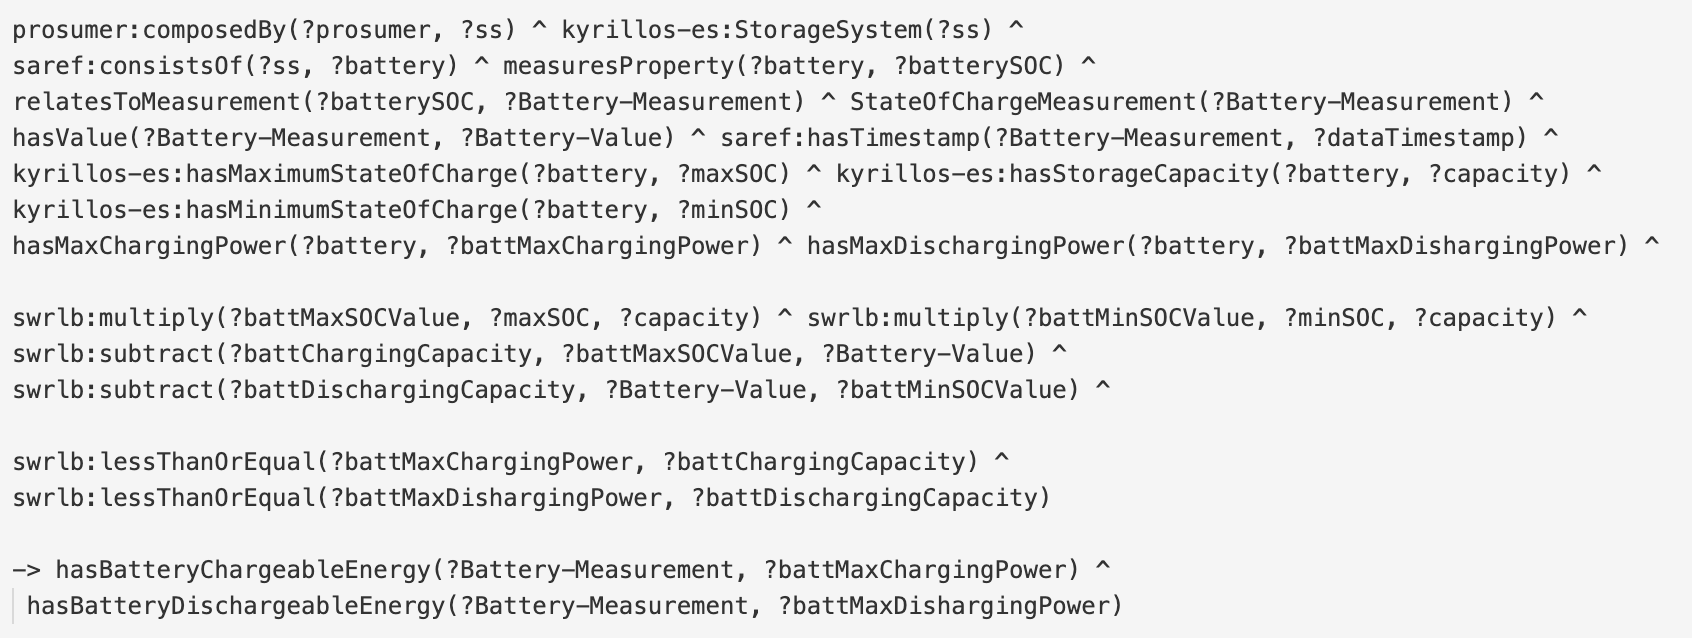
\includegraphics[width=15cm]{images/both <=.png}
    \caption{Screenshot della prima regola.}
    \label{fig:bothlessorequal}
\end{figure}


\subsection{Energia potenzialmente assorbibile = potenza massima di carica e Energia potenzialmente fornibile = capacità di scarica}
[\ref*{fig:charginglessorequal}]  Anche in questo caso la batteria può assorbire al massimo la potenza massima di carica siccome è inferiore o uguale alla capacità di carica,
e invece può fornire al più la capacità di scarica, perchè la potenza di scarica risulta maggiore della capacità.


\begin{figure}[H]
    \centering
    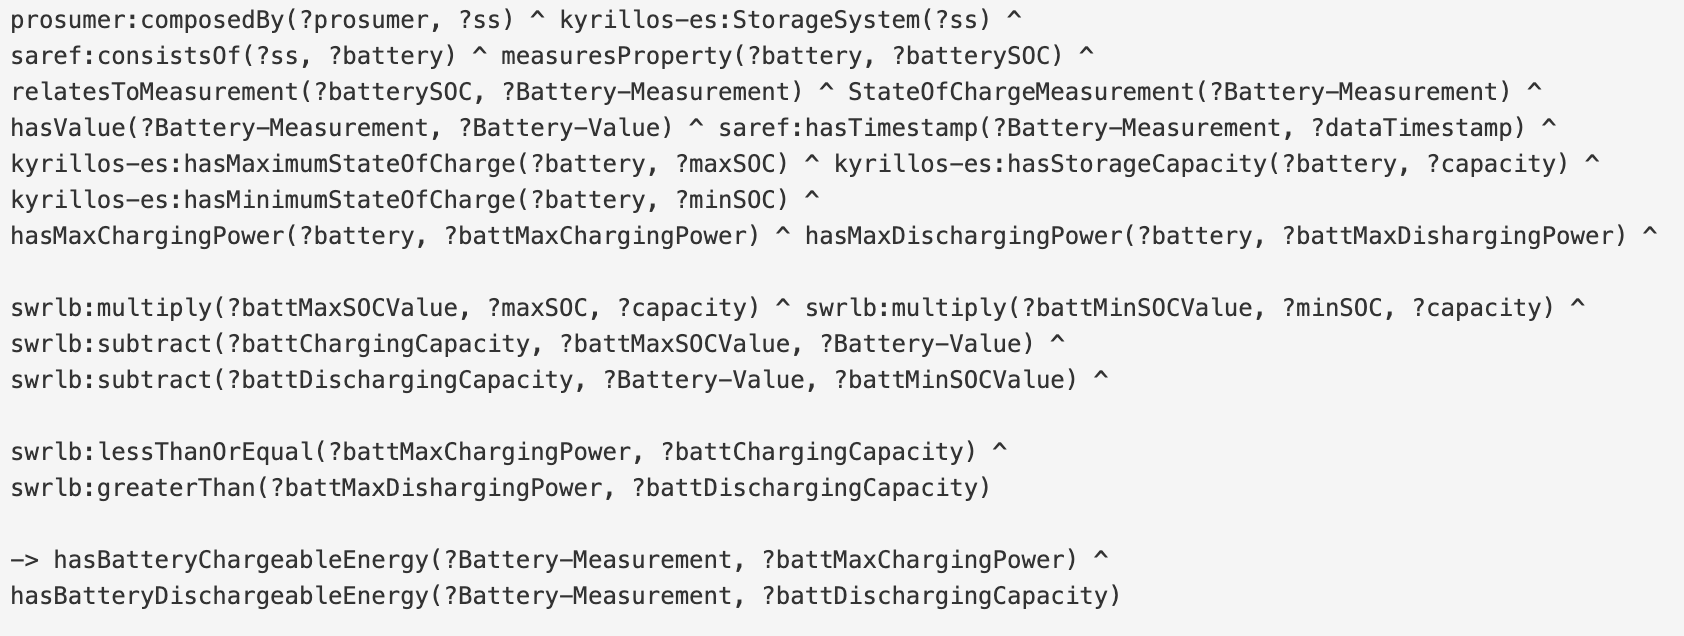
\includegraphics[width=15cm]{images/charging <=.png}
    \caption{Screenshot della seconda regola.}
    \label{fig:charginglessorequal}
\end{figure}


\subsection{Energia potenzialmente assorbibile = capacità di carica e Energia potenzialmente fornibile = potenza massima di scarica}

[\ref*{fig:charginggreater}] In questo caso invece, la capacità di carica è inferiore alla potenza massima, dunque la batteria può assorbibile al massimo la capacità di carica,
mentre può fornire al più la potenza massima di scarica, perchè inferiore o uguale alla capacità di scarica.

\begin{figure}[H]
    \centering
    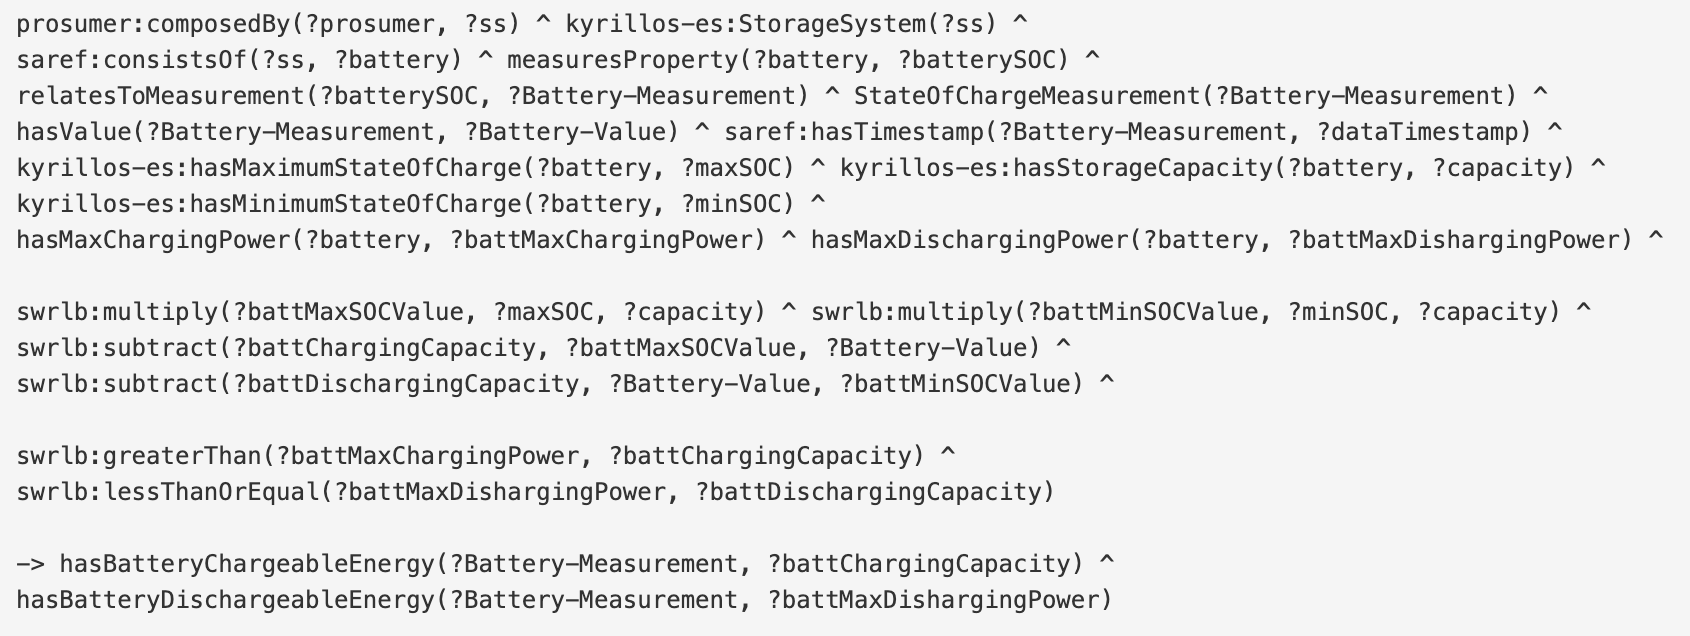
\includegraphics[width=15cm]{images/charging >.png}
    \caption{Screenshot della terza regola.}
    \label{fig:charginggreater}
\end{figure}

\subsection{Energia potenzialmente assorbibile = capacità di carica e Energia potenzialmente fornibile = capacità di scarica}

[\ref*{fig:bothgreater}] Infine c'è il caso in cui la potenza massima sia di carica che di scarica, siano superiori alle rispettive capacità che diventano dunque i valori massimi assorbibili o fornibili dalla batteria.

\begin{figure}[H]
    \centering
    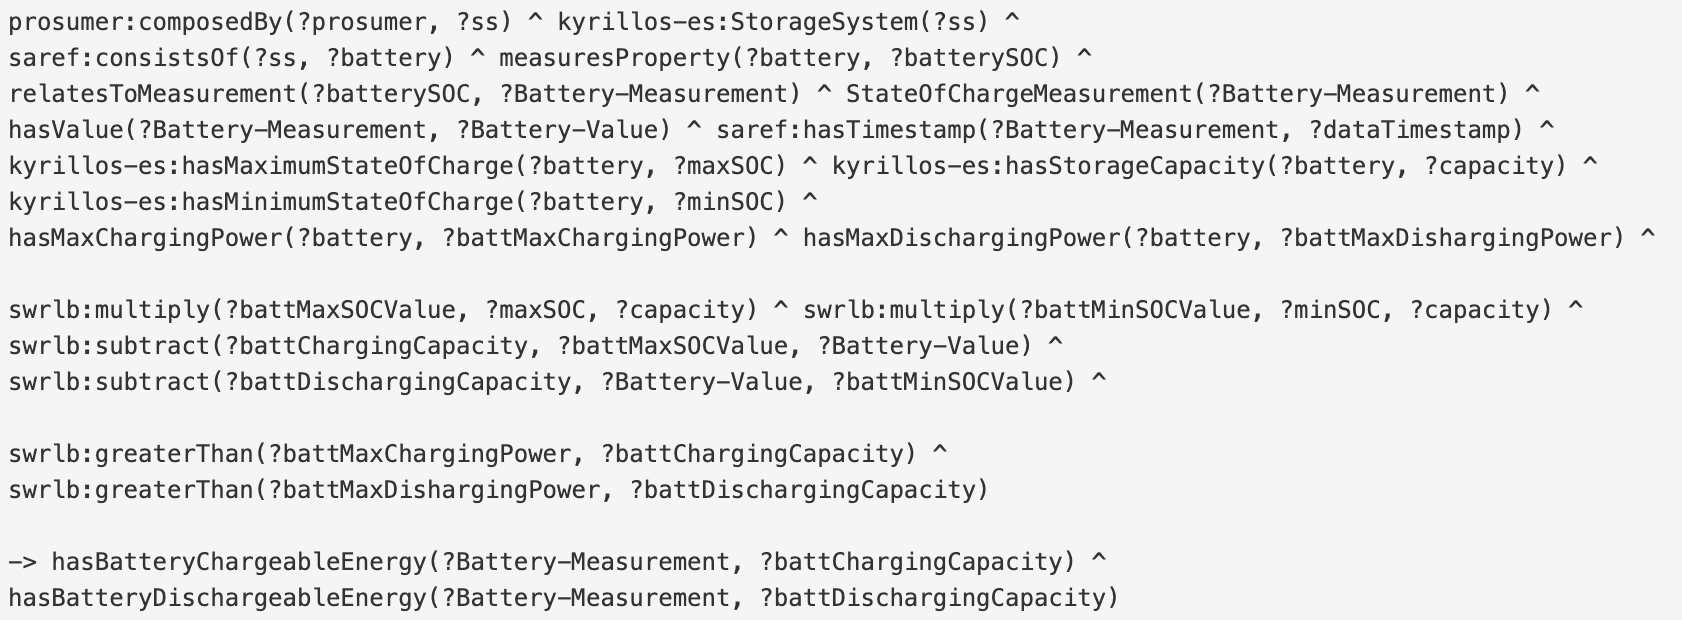
\includegraphics[width=15cm]{images/both >.png}
    \caption{Screenshot della quarta regola.}
    \label{fig:bothgreater}
\end{figure}

\section{SPARQL}\label{sec:sparql}
Nella seguente sezione verranno mostrate le query SPARQL e relativi risultati applicati agli individui creati nell'ontologia.

Si nota che per praticità, in quanto query molto lunghe, verranno mostrate solamente parti delle query come screenshot e i risultati, mentre le query complete sono disponibili nei relativi file di testo che verranno mostrati.


\subsection{PREFIX}
Per leggibilità i prefissi utilizzati per le query SPARQL verranno visionati solamente in questa sezione, siccome ripetitivi per ogni query.

Si può quindi notare l'utilizzo in particolare dell'ontologia \textit{battery}, la nuova ontologia \textit{prosumer}, con anche \textit{SAREF} e \textit{Interconnect}.

\begin{figure}[H]
    \centering
    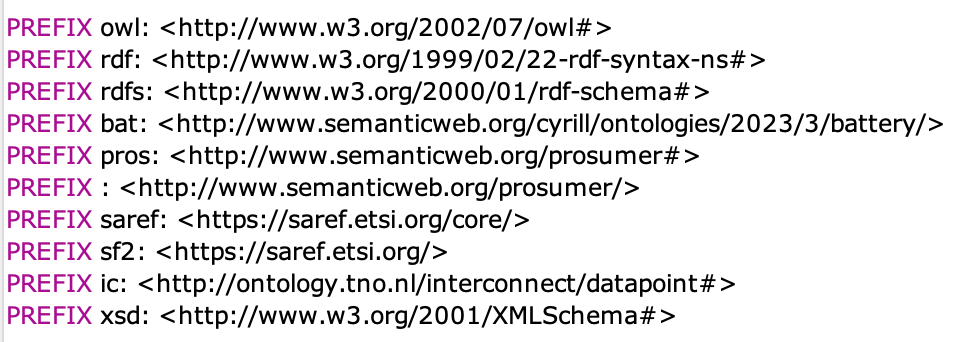
\includegraphics[width=15cm]{images/prefissi.png}
    \caption{Prefissi da anteporre alle query sull'ontologia.}
    \label{fig:prefix}
\end{figure}

\subsection{Query che calcola l'energia che può fornire o assorbire uno Storage System} \label{subquery}

Dato uno Storage System composto da una o più batterie, si vuole calcolare l'energia che il sistema nel suo complesso può assorbire o fornire.

Questa query in pratica utilizza i valori di energia precedentemente calcolati con le regole SWRL, e raggruppa per ogni intervallo di tempo quelli di tutte le batterie presenti nello Storage System del prosumer, in modo da ottenere l'energia che l'intero Storage System può assorbire o fornire.

\begin{figure}[H]
    \centering
    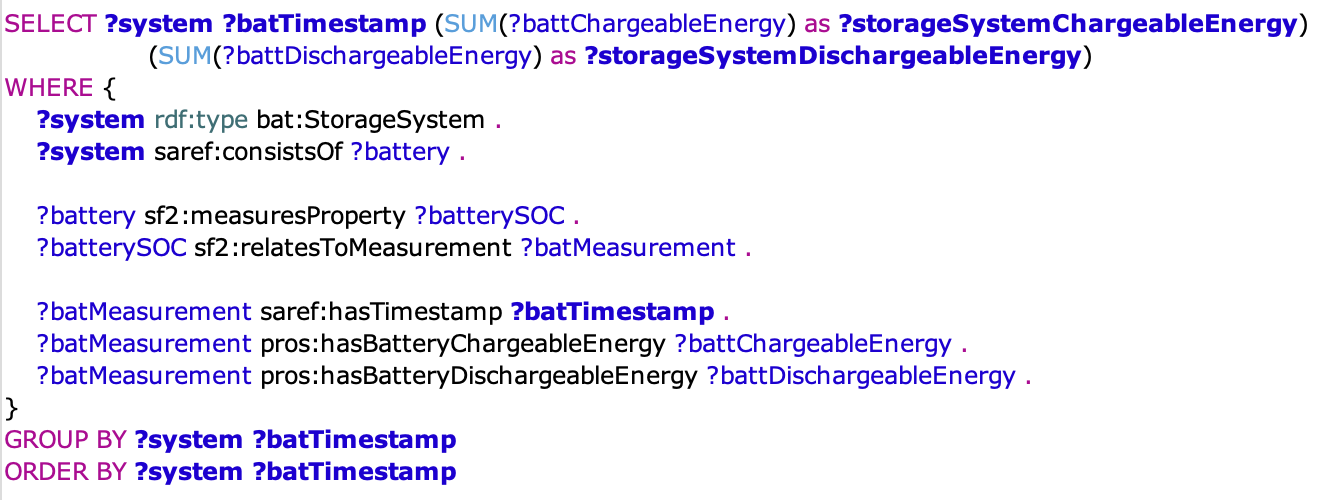
\includegraphics[width=15cm]{images/subquery.png}
    \caption{Query per il calcolo dell'energia che uno Storage System può assorbire o fornire.}
    \label{fig:subquery}
\end{figure}

La query è disponibile nella repository di \href{https://github.com/19eddie/SemanticWeb-Assignment02-03}{Github} nel file \href{https://github.com/19eddie/SemanticWeb-Assignment02-03/blob/main/SPARQL%20energia%20che%20pu%C3%B2%20assorbire%20o%20fornire%20uno%20StorageSystem.txt}{\textit{SPARQL energia che può assorbire o fornire uno StorageSystem.txt}}

Dall'esecuzione della query otteniamo dunque la quantità di energia che ogni Storage System può assorbire e immettere nel relativo timestamp. \ref{fig:subquery_res}

\begin{figure}[H]
    \centering
    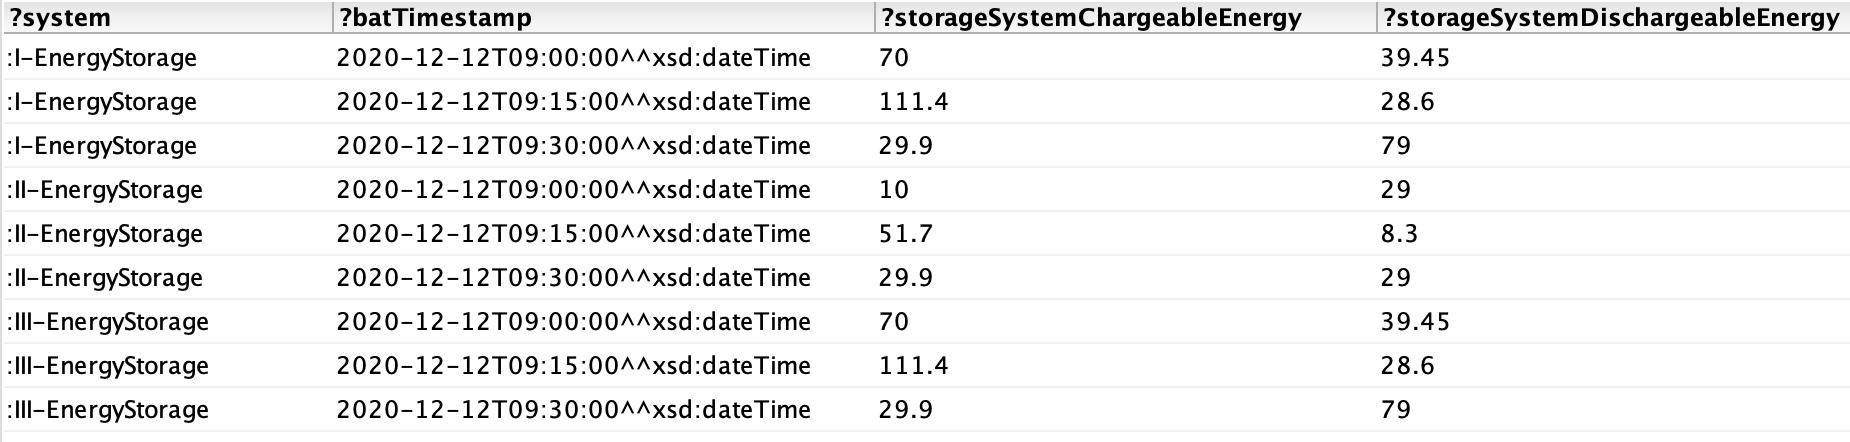
\includegraphics[width=15cm]{images/subquery_res.png}
    \caption{Risultati della query per il calcolo dell'energia che uno Storage System può assorbire o fornire.}
    \label{fig:subquery_res}
\end{figure}

\subsection{Query sul calcolo della flessibilità del contatore M1}

Con flessibilità di M1 si intende indicare il valore minimo e il valore massimo che il contatore può assumere in un determinato intervallo di tempo.
Il valore dipende nello specifico dalle caratteristiche del sistema di accumulo, dal carico richiesto e dalla quantità di energia prodotta dal generatore.
\begin{itemize}
    \item \texttt{M1 minimo:} la batteria viene caricata prelevando energia anche dalla rete;
    \item \texttt{M1 massimo:} la batteria non viene caricata e se il carico è maggiore della produzione, la batteria fornisce energia al carico.
\end{itemize}

\begin{figure}[H]
    \centering
    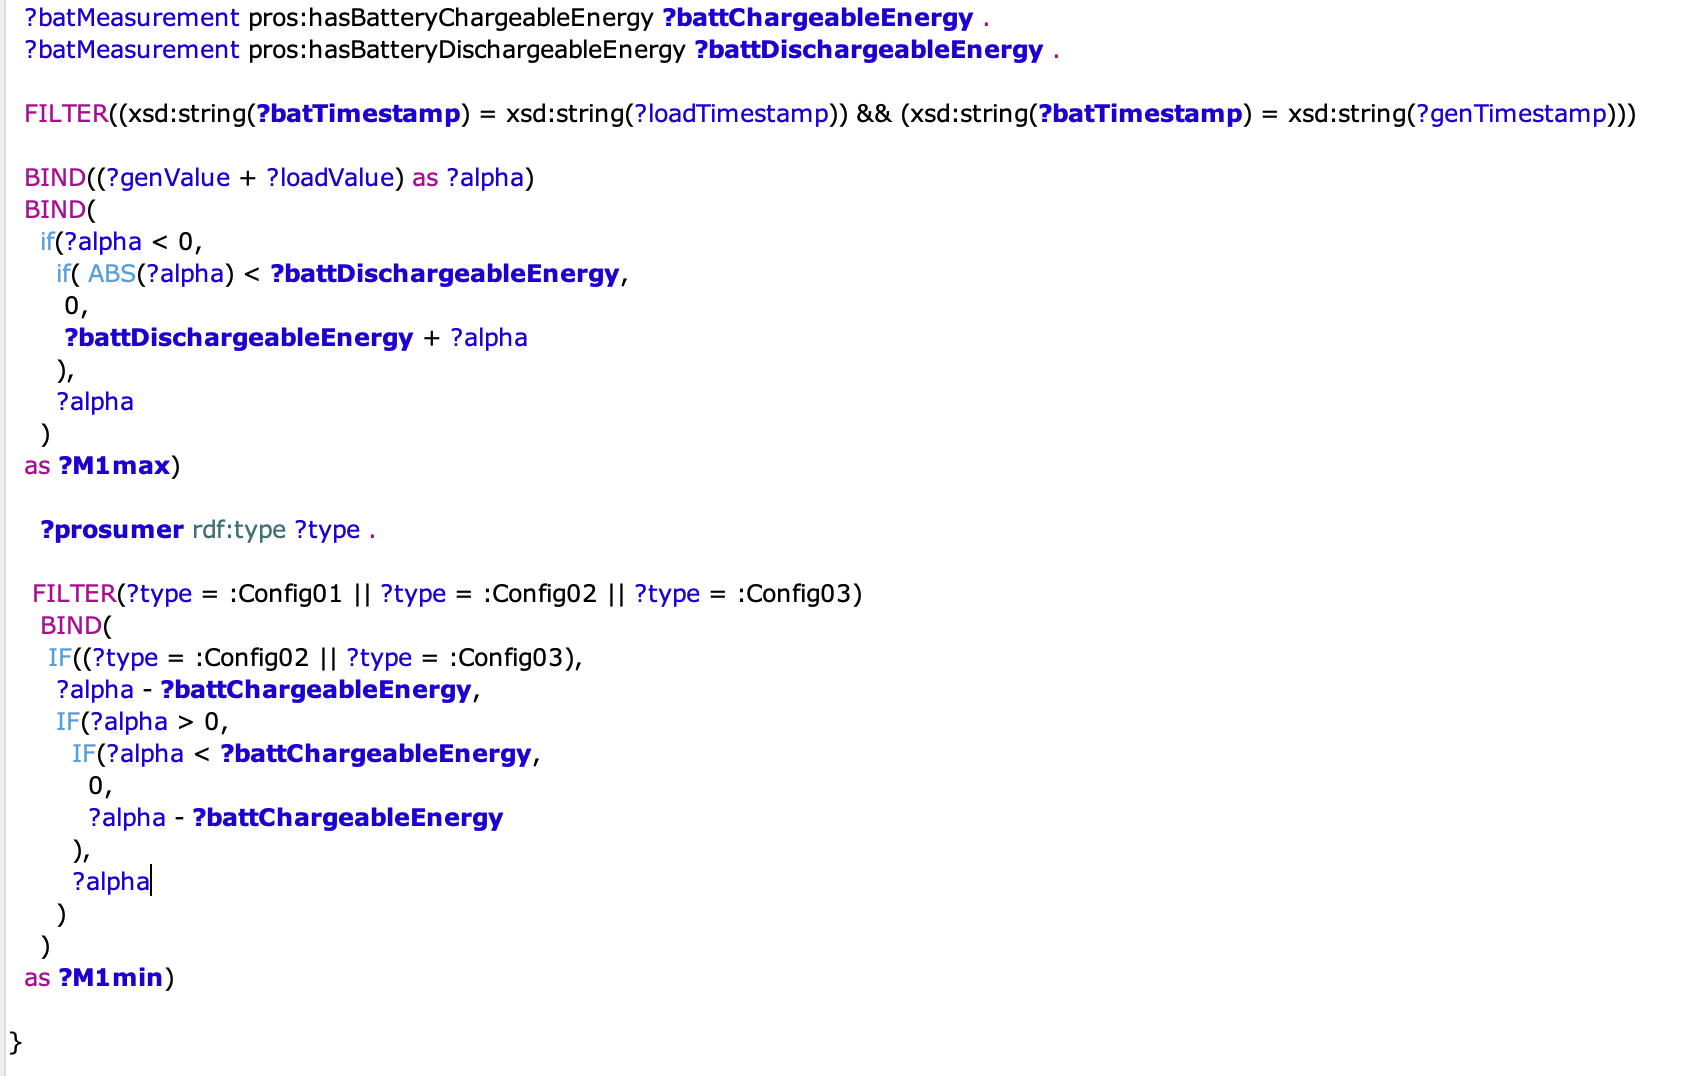
\includegraphics[width=15cm]{images/query_flessibilita.png}
    \caption{Query per il calcolo della flessibilità del contatore M1.}
    \label{fig:query_flessibilita}
\end{figure}

La query utilizza i valori di energia potenzialmente assorbibile o fornibile calcolati con le regole SWRL precedentemente descritte.
Si vuole notare che la query per come è presentata nel file \href{https://github.com/19eddie/SemanticWeb-Assignment02-03/blob/main/SPARQL%20flessibilit%C3%A0.txt}{SPARQL flessibilità.txt} 
purtroppo calcola la flessibilità di ogni batteria, e non di ogni Storage System.
Ciò è dovuto al software che è stato utilizzato per l'implementazione dell'ontologia e l'esecuzione delle query, ovvero Protègè,
che non supporta le subquery nel linguaggio SPARQL \cite{issueprotege}.
Nel caso in cui invece si utilizzasse un software che supporta le subquery, si potrebbe calcolare la flessibilità di ogni Storage System semplicemente inserendo la query \ref{subquery} come subquery e utilizzando quindi \textit{storageSystemChargeableEnergy} e \textit{storageSystemDischargeableEnergy} al posto di \textit{batChargeableEnergy} e \textit{batDischargeableEnergy}.
Ciò vale anche per le query successive.

\begin{figure}[H]
    \centering
    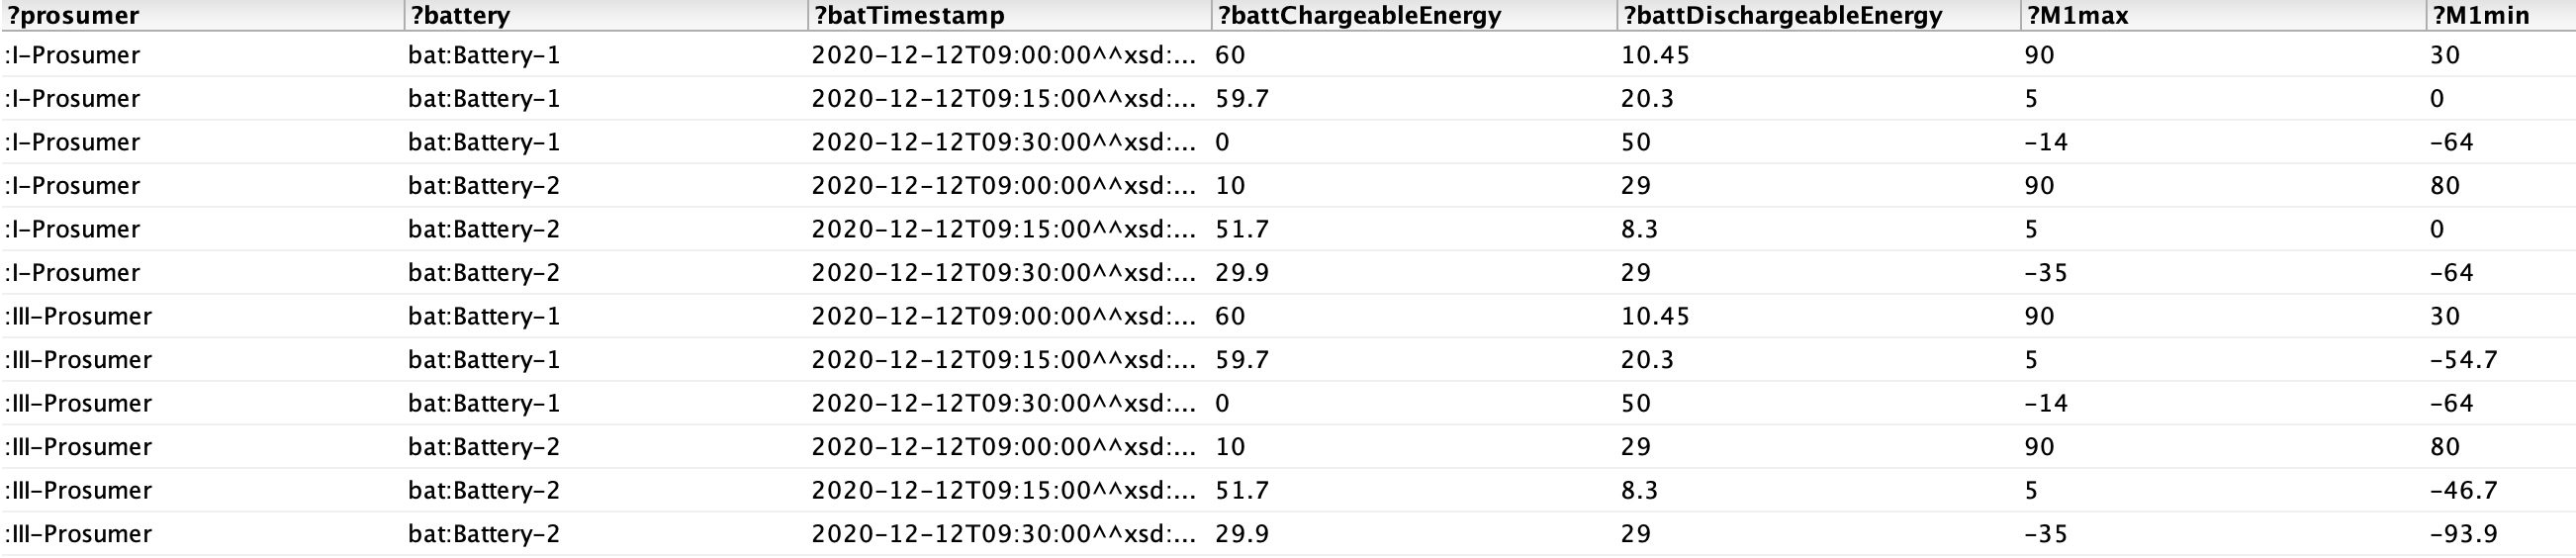
\includegraphics[width=15cm]{images/query_flessibilita_res.png}
    \caption{Risultati della query per il calcolo della flessibilità del contatore M1.}
    \label{fig:query_flessibilita_res}
\end{figure}

Si nota che se il valore di M1 è negativo, indica che l'energia è assorbita dalla rete; se è positivo, indica che l'energia è immessa nella rete.

\subsection{Logica per l'utilizzo del sistema di accumulo}
Per quanto riguarda la logica di come verranno calcolati i valori dei contatori nelle seguenti query, sono stati individuati i seguenti quattro casi:
\begin{itemize}
    \item \texttt{CASO 1:} il generatore produce meno energia di quella richiesta dal carico, la batteria è in grado di fornire quella mancante. Non viene prelevato o immesso nulla nella rete;
    \item \texttt{CASO 2:} il generatore produce meno energia di quella richiesta dal carico, la batteria non è in grado di fornire tutta quella mancante ma fornisce comunque tutta quella che può. Viene prelevato il restante dalla rete;
    \item \texttt{CASO 3:} il generatore produce più energia di quella richiesta dal carico, la batteria è in grado di assorbire tutta quella in eccesso. Non viene prelevato o immesso nulla nella rete;
    \item \texttt{CASO 4:} il generatore produce più energia di quella richiesta dal carico, la batteria non è in grado di assorbire tutta quella in eccesso ma assorbe comunque tutta quella che può. Viene immesso il restante nella rete.
\end{itemize}

\subsection{Query per il calcolo di M1 e M2 in prosumer di configurazione 1 e 2}

Le premesse sono le precedenti della query per il calcolo della flessibilità.

Questa query è inerente a prosumer di configurazione 1 e 2, ovvero prosumer che non presentano il contatore M3, in quanto i calcoli sono diversi come sarà mostrato in seguito.

Per entrambe le configurazioni, l'obiettivo è determinare come il sistema di accumulo (batteria) può essere utilizzato per fornire o assorbire energia
in base al carico equivalente e alla produzione di energia del generatore.

\begin{figure}[H]
    \centering
    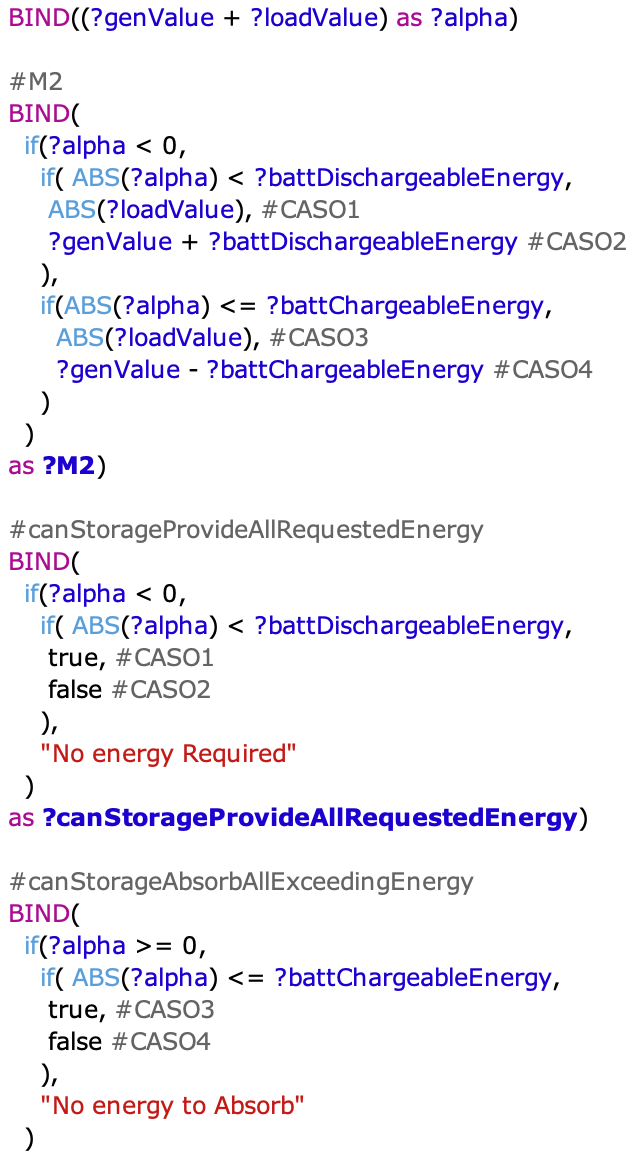
\includegraphics[width=6cm]{images/query_m1m2_config0102.png}
    \caption{Query per il calcolo di M1 e M2 in prosumer di configurazione 1 e 2.}
    \label{fig:query_m1_m2}
\end{figure}

Il calcolo di M2 dipende dal valore di alpha, la differenza tra la generazione di energia e il consumo.

Se alpha è negativo, viene richiesta energia dalla batteria. Se la batteria ha abbastanza energia da fornire, viene soddisfatta tutta la richiesta; altrimenti, viene prelevata il massimo possibile dall'energia del generatore e dalla batteria.
Se alpha è positivo, il prosumer produce più energia di quella richiesta. Se la batteria ha abbastanza capacità di carica, viene utilizzata per assorbire tutta l'energia in eccesso; altrimenti, la batteria viene caricata con il massimo possibile.
Nel calcolo di M1, il valore rappresenta l'energia totale scambiata con la rete, includendo l'energia del generatore, l'energia prelevata e fornita dalla batteria e l'energia assorbita o immessa dalla rete.
M1 viene ottenuto sommando il valore di M2 al consumo.

\begin{figure}[H]
    \centering
    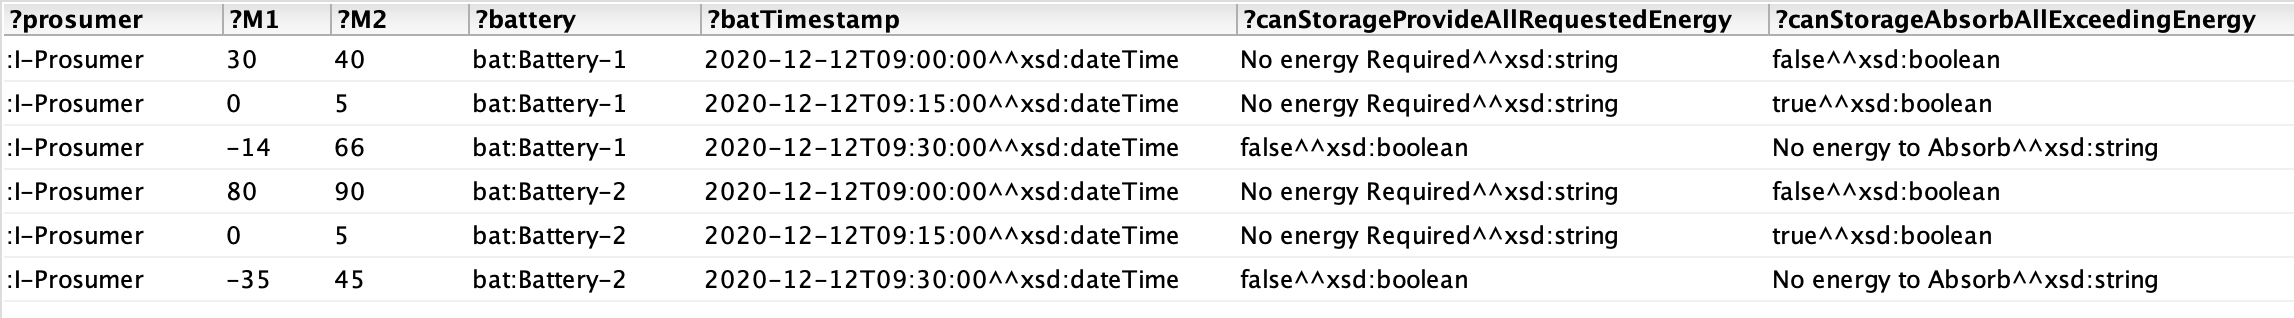
\includegraphics[width=15cm]{images/query_m1m2_config0102_res.png}
    \caption{Risultati della query per il calcolo di M1 e M2 in prosumer di configurazione 1 e 2.}
    \label{fig:query_m1_m2_res}
\end{figure}

La query completa si trova nel file \href{https://github.com/19eddie/SemanticWeb-Assignment02-03/blob/main/SPARQL%20M1%20e%20M2%20in%20config01%20e%20config02.txt}{\textit{SPARQL M1 e M2 in config01 e config02.txt}}.

\subsection{Query per il calcolo di M1, M2 e M3 in prosumer di configurazione 3}

Infine si vuole calcolare M1, M2 e M3 per prosumer di configurazione 3.

M2 rappresenta l'energia prodotta dal generatore, mentre M3 rappresenta l'energia scambiata con la batteria ed è determinata dalla differenza tra l'energia prodotta dal generatore e l'energia assorbita dal carico del prosumer.
Se il prosumer richiede energia dalla batteria, M3 assume il valore dell'energia richiesta, a meno che la batteria non abbia abbastanza energia disponibile, in tal caso assume il massimo di energia scaricabile dalla batteria. Se il prosumer produce più energia di quella richiesta,
M3 assume il valore dell'energia in eccesso che può essere assorbita dalla batteria, a condizione che abbia abbastanza capacità di carica; altrimenti, assume il massimo valore di capacità di carica della batteria, ma negativo.
Infine, M1 rappresenta il totale di energia scambiata con la rete, includendo l'energia prodotta dal generatore, l'energia scambiata con la batteria e il valore del carico del prosumer.

\begin{figure}[H]
    \centering
    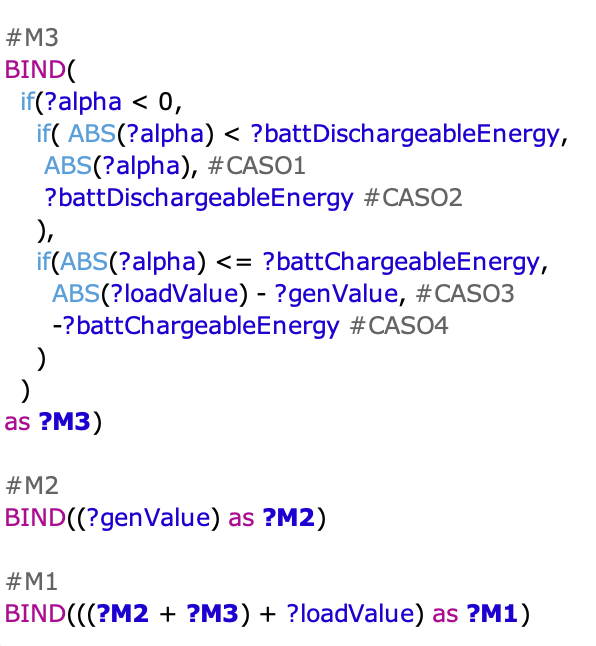
\includegraphics[width=7cm]{images/query_m3.png}
    \caption{Query per il calcolo di M1, M2 e M3 in prosumer di configurazione 3.}
    \label{fig:query_m3}
\end{figure}

La query completa si trova nel file \href{https://github.com/19eddie/SemanticWeb-Assignment02-03/blob/main/SPARQL%20M1%2C%20M2%2C%20M3%20in%20config03.txt}{\textit{SPARQL M1, M2, M3 in config03.txt}}.


\begin{figure}[H]
    \centering
    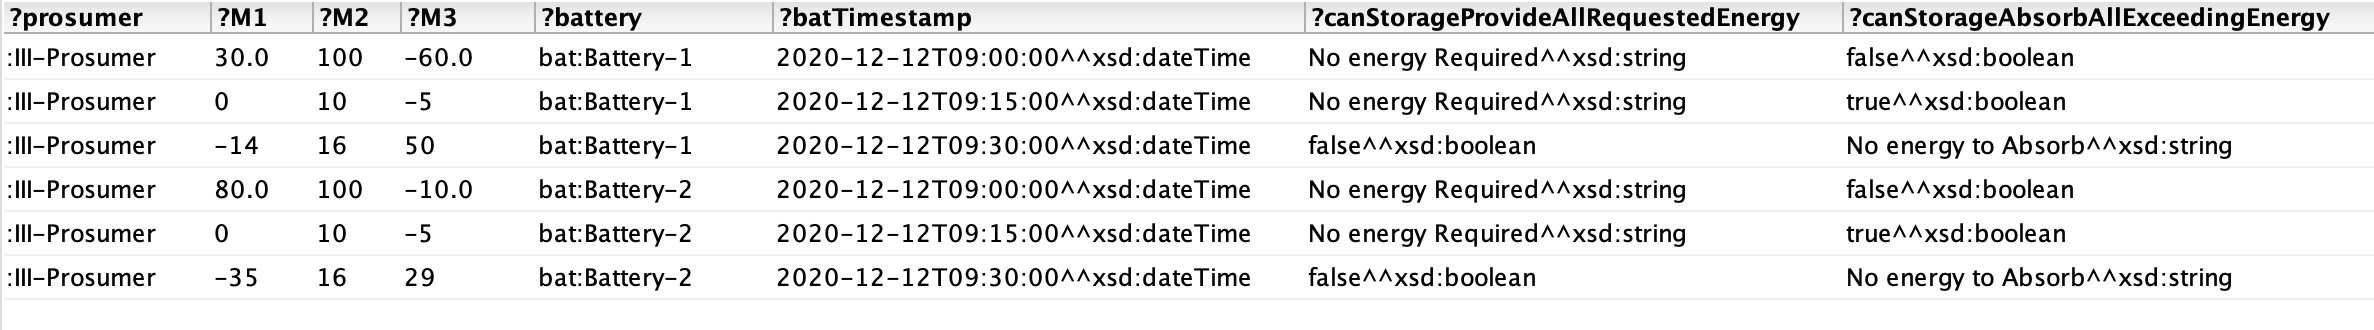
\includegraphics[width=15cm]{images/query_m3_res.png}
    \caption{Risultati della query per il calcolo di M1, M2 e M3 in prosumer di configurazione 3.}
    \label{fig:query_m3_res}
\end{figure}